\section{Tuning Decoding Parameters}
\label{chap:tuning-params}

In this section, I will cover the process of parameter tuning/optimization, regarding each of our decoding algorithms. We will examine the ideal configuration for maximizing each algorithm's effectiveness on our metrics, in an attempt to find the locally optimal configuration for our particular task, i.e. (rap) lyric generation. As it is with tuning ML models, the tuning process for decoding algorithms is not necessarily straight forward, and is similar to the way most neural networks themselves are trained, using gradient decent. As to make the process as thorough as possible, we will initialize it by choosing a broad range of starting parameter configurations. From there we will slowly narrow the field of configurations, ultimately leaving us with the most suitable parameters for the task at hand.

As we are dealing with a character-based language model, the initial metrics we are going to evaluate the parameters on are fairly basic text-evaluation criteria, as text coherence, including spelling, is not a given. It should also be noted that while the decisions regarding the parameters chosen largely informed by the metrics used, manual evaluation of the produced text is also part of the iterative testing process, for every single model (examples of which will be given below). This mirrors many other approaches in determining the best parameter values, as there is rarely a one-size-fits all. This approach is also supported by the aforementioned simplicity of our models, and the ease with which a human evaluator can discern gibberish from real text. Rather as being the entire basis of our choices, the metrics employed in this section should be thought of as more of an initial hint to what we are seeing, and always requiring closer examination. We also perform a simple pre-processing step, stripping the text of punctuation, as we are currently just intent on gauging the parameterized model’s ability to produce real words and sentences, the syntax being less important (for now). For more information on the evaluation criteria, see section \cref{sec:initial-eval-metrics}.

All tests will follow roughly the same iterative tuning process, usually consisting of 2 stages. First, a range of suitable values would be selected for each parameter. Prior to evaluation, V random seed values would be retrieved, equalling the number of iterations, as to level the playing field for the different configurations Then, each value would be used to generate V verses with C tokens, generally in the shape $20x200$.  When the generating had finished, the resulting text would be evaluated through plotting the examined metrics, and manually assessing the generated text. While the sample size was certainly not conclusive, they gave a suitable indication as to which values were the most promising, and which could safely be eliminated. After the elimination, the evaluation process would move on to stage 2 in which a new set of parameters would be selected on the basis of stage 1, and the process would be repeated, but now with a substantially higher number of iterations, usually increasing thrice over from 20 to 60. After the second stage, the set of parameter configurations would be reduced down to 1-3 configurations, which would then be used in the future global evaluation.

After evaluating the chosen "optimal" configurations against one another, we will examine the performance of each scheme and its configuration(s) over a broader set of metrics, to gauge their the strengths and weaknesses, and, if possible, further narrow the range of configurations. Afterwards, we will be examining the \textit{potential} of the different configuration, both positively and negatively, to create lyrics. This means examining the best and worst performing verses, with regards to our metrics, and seeing how they stack up against one-another. Creativity-wise, this approach does in some sense mirror the creative writing process of rappers, as it can be thought of as, in the case of testing the top-performing lyrics, as cutting off they stuff that never makes it to the record. All rappers undoubtedly produce a far greater amount of lyrics, than just what is released, as the majority having either been altered, completely re-written or discarded entirely. This makes for an arguably more a "fair" comparison between the actual lyrics and the generated text, as only a subsection of the best lyrics are included, and also gives us a chance to gauge the consistency of each model.

\subsection{Beam Search}
\label{sec:tuningbeam}

\begin{figure*}[ht!]
    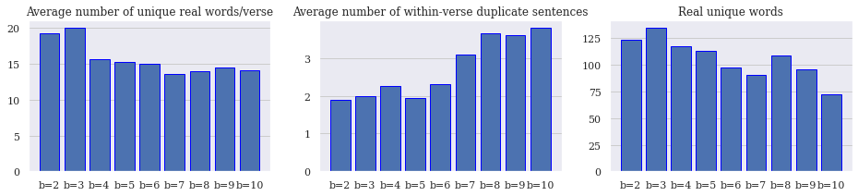
\includegraphics[width=\textwidth, keepaspectratio=true]{figures/beam_param_eval_s1.png}
    \caption{Beam Search Parameter Evaluation Metrics (Stage 1/2)}
    \label{fig:beamparameval_s1}
\end{figure*}

\begin{figure*}[ht!]
    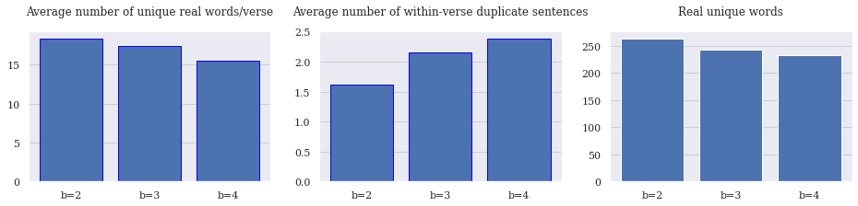
\includegraphics[width=\textwidth, keepaspectratio=true]{figures/beam_param_eval_s2.png}
    \caption{Beam Search Parameter Evaluation Metrics (Stage 2/2)}
    \label{fig:beamparameval_s2}
\end{figure*}

When optimizing beam search, we have a single parameter we can tune, namely the beam width ($\beta$). For our initial fine-tuning, we tested the on the parameter configurations seen in Table 5 with $\beta=[2\dots10],step=1$. For each of the 9 configurations, I based the evaluation metrics on $20x200$ tokens, totalling $4k$ tokens for each configuration, $36k$ in total.

Looking at the results of the initial tests in \cref{fig:beamparameval_s1}, we can see that regardless of which metric we are looking at, quality diminishes at $\beta < 4$, with $\beta = \{2, 3, 4\}$ being the best performers. Especially text generated with $\beta = [7 \ldots 10]$ seems to be performing badly, according to our metrics. On the basis of these results, we are going to move on with $\beta = \{2, 3, 4\}$. Now that we have eliminated two thirds of our configurations, let us generate text only using the remaining parameters, this time upping the number of iterations from 20 to 60. We will still be generating 200 tokens each time, totalling 12k tokens per value of $\beta$, 36k tokens overall.

In \cref{fig:beamparameval_s2} we roughly get the tendencies we saw in the initial exploration confirmed, the main difference being that $\beta=2$ has overtaken $\beta=3$ on every parameter, having a larger number of unique real words per verse, a larger vocabulary and, most noticeably, a substantially larger  number of within verse duplicate lines. This improvement confirms the usefulness of performing the same tests on a larger body of text, as looking solely at the first parameter evaluation, would have suggested that $\beta=3$ would be the preferable value, moving forward. In conclusion we discovered that $\beta=2$ was the optimal value for our model and dataset, making it the value of choice moving forward.

\subsection{Temperature Sampling}
\label{sec:tuningtemp}

The next decoding scheme up for parameter exploration is temperature sampling. As with beam search, we only having 1 parameter to explore, namely temperature. Here, we will be testing the temperature values $T=[0.1 \ldots 1.2]$ with a step size $s=0.1$, equalling 12 different temperatures. Each temperature will be tested with 4k generated tokens per value of T, totalling 48k tokens.

After the first exploration stage, as can be seen in Appendix II, we can conclude that $T=[0.5 \ldots 0.9]$ gives us the largest number of unique real words, the average starting to drop off at $T>0.9$. It is worth mentioning that the similar values of average number of unique real words we see around $T=0.3$ vs $T=1.2$ tell very different stories, if we take a closer look.

Looking at the two generated texts, using the same seed, in \cref{tab:temperatureexample}, the difference between them is very evident. The text generated at the low temperature (Text 1), bears a lot of resemblance to text generated by our deterministic models, in that it is very repetitive, resulting in it having low average unique words/verse, many of the words being identical. Moving on to the lyrics generated by with a high temperature (Text 2), we are presented with a wholly different story. Instead of seeing repetitions, we are seeing a text made up of almost exclusively unique “words”. However, what it makes up for in avoiding repetition, it unmistakably pays for in that many of the words being complete gibberish. While Text 2 has 38 “words”, 36 of which are unique ($\sim95\%$), many of them to the degree of no longer being actual words. In comparison, Text 1 has a pitiful 11 unique words out of 49 ($\sim22\%$), yet every single one of those words are actual, real words. And while the number of real words in Text 2 still dwarfs that of Text 1 (29 vs. 11), the syntactic structure of Text 1 is certainly the superior, being error-free. This highlights one of the aforementioned shortcomings of the metrics for our initial parameter exploration, further stressing the importance of these metrics merely being an initial approximation.

\begin{table*}[htb!]
    \begin{center}
    \caption{Example of Temperature Sampling (\textbf{EXPLICIT CONTENT})}
    \vspace{6pt}
    \bgroup
    \def\arraystretch{1.5}
    \label{tab:temperatureexample}
    \begin{tabular}{|l|l|}
        \hline
        \multicolumn{1}{|c|}{\textbf{Text 1 (T=0.3)}} & \multicolumn{1}{|c|}{\textbf{Text 2 (T=1.2)}} \\\hline
        \textit{i don’t know how to face it} & \textit{make a pac joint’ly seettme}\\
        \textit{i don’t know how to face it} & \textit{which niggas drone and it’d}\\
        \textit{i don’t know how to face it} & \textit{rell,}\\
        \textit{i don’t know how to face it} & \textit{bigger pay struggle but my}\\
        \textit{i don’t know how to face it} & \textit{rostogues i blow that}\\
        \textit{you can let it out} & \textit{okay old fat 2pac}\\
        \textit{you can let it out} & \textit{kana,  might hit your bitch by}\\
        \textit{you can let it} & \textit{fast like i spray drass}\\
        & \textit{tell a nigga}\\\hline
    \end{tabular}
    \egroup
    \end{center}
\end{table*}

After examining all the metrics, I choose to move on to stage 2 with 5 different parameter specification $T=[0.5\ldots0.9]$. The reason behind choosing 5, as opposed to the 3 we choose last time, was that the benefit differences between the temperatures are not as obvious. Because of this, we would rather include more values include more values rather than less in our stage 2 testing, on the off chance that the extreme values $T=\{0.3,0.9\}$ turn out to be superior, given a greater sample size.

After running stage 2 of the evaluation, two parameter values in particular seem to be outperforming the rest, namely $T=\{0.7,0.8\}$.  They both have the best number of unique real words per verse, some of the lowest within-verse duplication scores and decently sized vocabularies. The main difference between the two versions is that, as we saw in \cref{tab:temperatureexample}, the higher temperatures will give us a greater number of nonsense words and sentences while the lower temperature will  give us a greater number of repetitive sentences; the familiar dilemma in character-based text generation. I ended up moving on with the consistently more coherent parameter, $T=0.7$ as I estimate that coherence is overall a more necessary feature, for our purposes. This does not mean that coherence is \textit{always} preferable over novelty, all things being equal, bur rather than a certain level of coherence has to be attained, for novelty to outweigh its importance.

\subsection{Top-k Sampling}
\label{sec:tuningtopk}

After temperature sampling we move on to top-k sampling, a method which also includes the temperature parameters, meaning that we are required to evaluate 2 different parameters. As parameters, we have chosen to test the same range of temperatures as we did with temperature sampling, and for values of k, we are testing $k=[2 \ldots 6],s=1$. This means that for top-k, we are testing $12 \cdot 5 = 60$ different values, 4k character each, totalling 240k characters.

Looking at \cref{fig:top-k-param-eval-1}, we can see that in terms of both average number of unique real words and number of real unique words, there is a tendency for it to start off well and the decrease over time. Regarding the duplicate sentences, however, the distribution almost seems random, with a slight average increase after $k>3$, indicating that this metric is likely not very useful for determining ideal values for k. This, in combination with manual evaluation of the generated text at higher values of k, we can eliminate values $k>3$, equalling 36 distinct parameter settings. No consistent drawbacks emerge with regards to temperature values, so as opposed to eliminating temperature values, we will proceed with the same range of values for $k=\{2,3\}$.

After stage 2, we continue to see $k=3$ perform consistently worse than $k=2$ on all parameters, and so we eliminate it from consideration. We now take a look at the remaining 12 values, all with $k=2$ and varying degrees of temperature. Looking at reduced version of our stage 2 tests in Appendix VI, the standout temperature values $T=\{0.6,0.7\}$, the former of the two winning in, as it produces fewer within-verse duplicate sentences. As previously mentioned, top k is generally speaking one of the most promising decoding techniques for language generation, so in contrast to the two previous methods, we retain both values for further evaluation.

\subsection{Nucleus Sampling}
\label{sec:tuningnucleus}

Our final decoding algorithm is nucleus sampling, generally believed to be the best decoding algorithm for text generation. Our stage one test parameters follow those of the previous methods, testing p¬ values $p=[0.90 \ldots 0.99],s=0.01$. However, due to a combination of this being our presumed best coding scheme, as well as the low number of different values tested (10), we up the sample size per configuring to  60 x 200 iterations. This increase ends up totalling 12k characters for each configuration, 120k overall, and it allows us some added certainty with regards the stability of our results, due to our sample size.

After our initial tests, as can be seen in \cref{fig:top-p-param-eval-s1}, we are left with possibly the most conclusive results so far, lower values of p scoring higher in in almost every single metric and higher p values performing exceptionally badly, even in comparison with other models. Looking at the data, we can immediately gather 2 things: firstly, not only are the higher values not performing well at all, but the lower ones seem to be improving the lower we go, which suggests that we should consider including even lower values of p. Secondly, even the top number configuring only scores an average of 22.85 number of real words per verse, which is low compared to our previous tests, reinforcing the idea of testing lower values of p. Drawing upon these findings, the configurations for stage 2 will consists of $p=[0.80 \ldots 0.89]$. This will allow us to gauge whether there is continual improvement to be found, in further lowering the p value, or whether a limit has been found.

\begin{figure*}[ht!]
    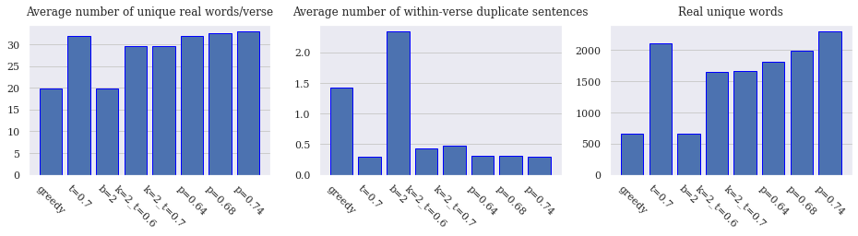
\includegraphics[width=\textwidth, keepaspectratio=true]{figures/combined_param_eval.png}
    \caption{Evaluation Metrics for Optimized Decoding Methods}
    \label{fig:combined-param-eval}
\end{figure*}

After \hyperref[fig:top-p-param-eval-s2]{stage 2} we see continue to see improvement of the number of unique real words per verse, as we continue to decrease p, the value slowly beginning to taper off at the very end. This improvement is also evident in inspecting the generated text, the output becoming increasingly fluent as interesting, while still suffering from some syntactic incoherence. Because of this, we will extend the testing to a continue to stage 3, in which we again decrease p, this time to $p=[0.70 \ldots 0.79]$.

After the \hyperref[fig:top-p-param-eval-s3]{3rd stage}, we start to see the vocabulary size slowly decreasing in tandem with p, after having either grown or stagnated for $p=[0.80 \ldots 0.99]$. As we would expect in lowering p, the number of within-verse duplicate sentences has also generally gone noticeably up, all but p=0.75 being larger than previously seen. However, the number of real unique real words has, while not as drastically as previously, continued to increase. Examining the lyrics, we also do still seem to be getting lyrics of higher quality, while duplication is still not very persistent. As the results as still partly inconclusive, as to which values perform the best, we will perform a final testing stage, this time employing $p=[0.5 \ldots 0.68],s=0.02$, increasing the step size to limit the number of configurations tested to 10, while still covering a large part of the spectrum.

Looking at the data from \hyperref[fig:top-p-param-eval-s4]{stage 4}, we now see a clear degradation in quality, in the form of repetition. Not only are the values for unique real words/verse decreasing noticeably, but so is the vocabulary size. As has been a theme throughout, the average number of within-verse duplicates, while very high for $p=\{0.50\}$, fluctuate heavily, indicating either that they are not very heavily related to our model parameter, or that the sample size is too small to accurately measure it.

To conclude the test, I have chosen to include configurations with $p=\{0.64,0.68,0.74\}$. I choose these values in particular, for a few reasons. Firstly, they represent the best part of the spectrum of our metrics, having a good balance between low repetition and high number of unique words per sentence. Secondly, they generated the most consistently good verses, again finding a nice balance between natural sounding language and a rich vocabulary.

\section{Results}
\label{chap:results}

Now that we have determined the parameters of our decoding schemes, we move on to our results, in which we will be pitting the different strategies and configurations up against one-another. For this evaluation, to properly measure the effectiveness of our different approaches, we generate lyrics with each configuration for 500 iterations of 200 tokens, totalling 100k tokens for each set of parameters. As with our parameter tuning in  \cref{chap:tuning-params} this is done using 500 distinct and ordered seeds within the generation loop, using the same collection of seeds for each generation. In this section, I also present a new set performance metrics, as to provide a fuller account of each configuration's potency. For more information on the these metrics, consult \cref{sec:other-eval-metrics}.

\subsection{Generating and Evaluating Lyrics}
\label{sec:gen+eval}

\begin{table}[H]
    \begin{center}
    \caption{Final Chosen Decoding Schemes}
    \vspace{6pt}
    \bgroup
    \def\arraystretch{1.5}
    \label{tab:chosen-decoding-methods}
    \resizebox{7cm}{!}{
    \begin{tabular}{|c|c|c|}
        \hline
        \textbf{Algorithm} & \textbf{Type} & \textbf{Parameter(s)} \\\hline\hline
        Greedy & Deterministic & \textit{N/A} \\\hline
        Beam Search & Deterministic & $\beta=2$ \\\hline
        Temperature & Stochastic & $t=0.7$ \\\hline
        Top-k & Stochastic & $k=2,t=0.6$ \\\hdashline
        Top-k & Stochastic & $k=2,t=0.7$ \\\hline
        Nucleus & Stochastic & $p=0.64$ \\\hdashline
        Nucleus & Stochastic & $p=0.68$ \\\hdashline
        Nucleus & Stochastic & $p=0.74$ \\\whline
    \end{tabular}
    }
    \egroup
    \end{center}
\end{table}

Looking at results of these generations via our initial evaluation metrics in \cref{fig:combined-param-eval}, we find that, as expected, the decoding schemes with the greatest number of repetitions, as can be seen in the large number of duplicate lines and comparatively small vocabularies and average number of real unique words, are the two deterministic decoding approaches: \textit{greedy} and \textit{beam} search. Interestingly, our beam search approach produces a substantially higher number of within-verse duplicates than the greedy search configuration, “beating” it by $\sim$0.91 duplicate lines on average, or $\sim$61,1\%. At the other end of the scale, we find our various different nucleus sampling configurations, as well as our simple temperature sampling method, all relatively close to one-another, across all the initial metrics. To better distinguish between their performance, let us take a look at another set of metrics, a bit more tailored towards general text evaluation.

\begin{figure*}[ht!]
    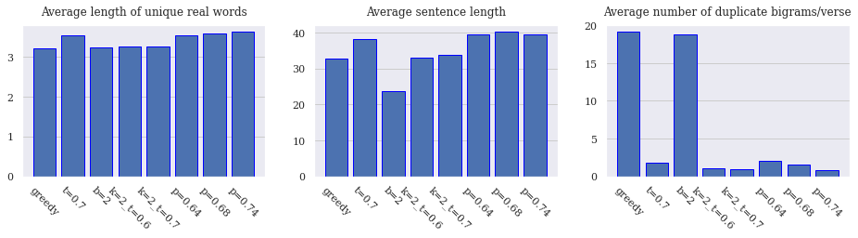
\includegraphics[height=\textheight, width=\textwidth, keepaspectratio=true]{figures/extended_combined_param_eval.png}
    \caption{Extended Evaluation Metrics for Optimized Decoding Methods}
    \label{fig:extended_metrics}
\end{figure*}

Taking a look at the first of the new metrics in \cref{fig:extended_metrics}, we can see that the configurations that are performing the best, are generally the as we saw before previously. This is also true for our $top-p, p=0.74$ configuration, which continues being one of the best performing configurations. However, while it manages an average real word length of 3.624, which \textit{is} better than the rest of our configurations, it is in stark contrast to the average word length of our RL dataset, which is $\sim$ 5.17.

Looking at the bigram duplicates per verse, it becomes quite evident that the repetition issue we discussed previously, is not limited to entire sentences, as was seen in \cref{fig:combined-param-eval}. For both greedy search and beam search, just under half of all bigrams within each verse are duplicates, further cementing their inadequacy for generating interesting lyrics, within in this context.

If we consider just the values for the stochastic decoding, as can be seen in \cref{fig:avg-bigrams} marked in in blue, the noticeable difference becomes much clearer, through removal of the vast outlier values in greedy- and beam search.

\begin{figure}[H]
    \centering
    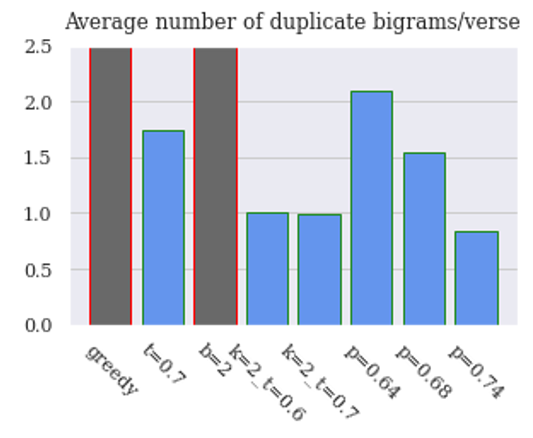
\includegraphics[scale=0.3,keepaspectratio=true]{figures/avg_bigrams.png}
    \caption{Average Duplicate Bigrams/verse}
    \label{fig:avg-bigrams}
\end{figure}

Our lower \textit{p} value actually produces twice the amount of duplicate bigrams/verse, in comparison to both $p=0.74$ as well as both top-k configurations. Also our mid nucleus configuration $p=0.68$ and our temperature sampling configuration $t=0.7$ suffer from the repetition issue, despite not quite as severely.

From looking at all the different metrics, let us now take a look at examples of the actual lyrics produced by the different configurations, all of which can be seen in full in \cref{tab:lyric-generation-examples}. Evidently, the repetition issues with both the greedy and beam search configurations are have persisted. Interestingly, each generation representation a different type of repetition, the greedy search example containing entirely duplicated lines and the beam search example duplicate words and bigrams, as can be seen in \cref{tab:repetition-issues}.

\begin{table}[H]
    \begin{center}
    \caption{Types of Repetiton Issues with Greedy Search and Beam Search}
    \vspace{5pt}
    \bgroup
    \renewcommand\cellset{\renewcommand\arraystretch{1.13}}
    \def\arraystretch{1.8}
    \label{tab:repetition-issues}
    \resizebox{7cm}{!}{
    \begin{tabular}{|m{1.5cm}|m{8.7cm}|}
        %\multicolumn{1}{c}{\textbf{Config}} & \multicolumn{1}{c}{\textbf{Generated Lyrics}}
        %\\
        \hline
        \makecell[c]{Greedy \\ Search} &
        {\em \makecell[l]{
        i want to get the police but i can't stop the same \\
        i don't know what i wanna do \\
        i don't know what i wanna do \\
        i don't know what i wanna do \\
        i don't know what i wanna do \\
        i don't know what i wanna d}} \\\hline
        \makecell[c]{Beam \\ Search \\ $\beta=2$} &
        {\em \makecell[l]{
        i want to tell you about it, i was the one that i know \\
        and i know it's just the way i escape \\
        yeah, i said it all falls down \\
        i don't know what to do \\
        they wonder why i never get tight \\
        i don't want}} \\\hline
    \end{tabular}
    }
    \egroup
    \end{center}
\end{table}

In the \textbf{greedy} search example, we get 1 line of actual rap, followed by 5 repeated lines which are completely identical, minus the missing o in the last line, which is due to the 200-character cut-off. In the \textbf{beam} search example, we do not have any duplicate lines, yet we have a lot of duplicate bigrams, and a lot of repeating words in general, such as: "i" (9 occurences). However, it is clear that \textbf{beam} search does do a better job of mimicking rap lyrics than greedy search and, despite its repetition issue, actually almost sounds plausible.

Something we would ideally have wanted to see some more of, in the example sentences, would have been rhymes, This is, however, just sample lines, so it is certainly possible that there is still some level of rhyme generation going on. For a fuller evaluation of the model’s general ability to rap lyrics specifically, let us take a look at the overall rhyme density of each of the configurations.

\begin{table}[H]
    \begin{center}
    \caption{Decoding Configurations - Rhyme Densities}
    \vspace{6pt}
    \label{tab:decoding-configs-rd}
    \bgroup
    \def\arraystretch{1.3}
    \resizebox{7cm}{!}{
    \begin{tabular}{l|c|c}
        Rank* & \multicolumn{1}{c|}{Configuration} & Rhyme Density \\[0.1cm]\hline
        1. (23.) & Top-k, $k=2, t=0.6$ & 1.055 \\
        2. (28.) & Top-k, $k=2, t=0.7$ & 1.047 \\
        3. (33.) & Temp Sampling, $t=0.7$ & 1.006 \\
        4. (36.) & Greedy Search & 0.994 \\
        5. (36.) & Beam Search, $\beta=2$ & 0.964 \\
        6. (36.) & Top-p, $p=0.64$ & 0.951 \\
        7. (36.) & Top-p, $p=0.68$ & 0.947 \\
        8. (36.) & Top-p, $p=0.74$ & 0.935 \\\hline
        \multicolumn{2}{c|}{Mean Rhyme Density:} & \textbf{0.987} \\\hline
        \multicolumn{3}{l}{\makecell[l]{* Parenthesized rank denotes the rank at which the \\ decoding configuration would have slotted in, amongst \\ all rappers}}
    \end{tabular}
    }
    \egroup
    \end{center}
\end{table}

Looking at \cref{tab:decoding-configs-rd}, it is evident that our model managed to learn to map rhymes, at least to a certain extent, as all of our models manage beat the worst and second-to-worst performing rapper, in terms of average rhyme density (Andre 3000: $RD=0.883$, Ice Cube: $RD=0.924$). While none of our models manage to reach the average RD threshold of the real MCs, they perform amicably, the top-scoring model top-k with $k=2, t=0.6$ scoring 1.055, which would land it at the 23rd position amongst the tested rappers. We can also observe that the models we previously perceived to be the best performers with regards with regards to producing legible text, both with regards to the tested metrics as well as the manual “eye-test” evaluation, are dead-last amongst our models in their average rhyme density.

Our temperature sampling configuration also still seems to be competing reasonably well, despite being one of the simpler algorithms, although it is still outperformed when also applying the \textit{top-k} coding scheme on top.

From all the metrics, we can gather that 3 of the sampling techniques shows promise in one or more areas of lyric generation, namely \textit{temperature sampling}, \textit{top-k sampling} and \textit{top-p sampling}. As a result of this, we will move on with these three techniques, consisting of 6 different configurations, to examine their peaks and valleys of their rhyming abilities. In these tests, we will move away from just looking at the total aggregate performance of each configuration, but instead examine the peaks and valleys of each configuration, to get a better idea each configuration's "potential", as well as how outliers might be influencing the results.

\subsubsection{Outliers and Performance Across the Spectrum}
\label{sec:outliers+performance-spectrum}

\begin{figure*}[ht!]
    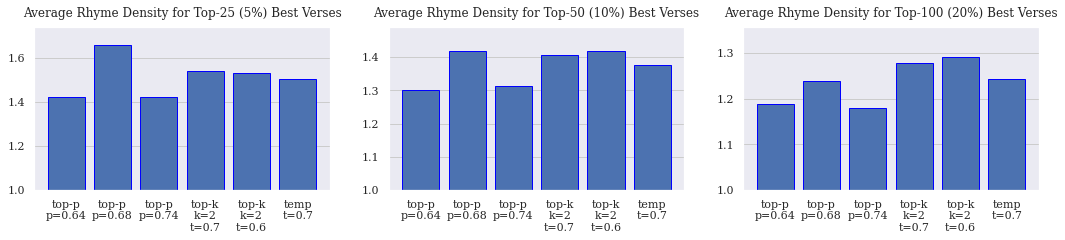
\includegraphics[height=\textheight, width=\textwidth, keepaspectratio=true]{figures/top_verse_rd.png}
    \caption{Average RD for Top-10, Top-25 and Top-50 Verses for Optimized Configurations}
    \label{fig:avg_rd_top}
\end{figure*}

\begin{figure*}[ht!]
    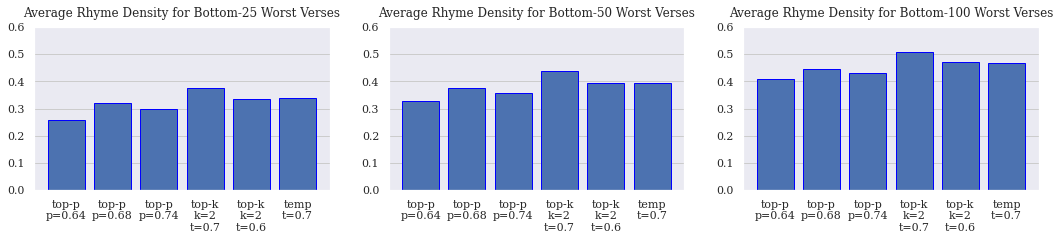
\includegraphics[height=\textheight, width=\textwidth, keepaspectratio=true]{figures/bot_verse_rd.png}
    \caption{Average RD for Bottom-10, Bottom-25 and Bottom-50 Verses for Optimized Configurations}
    \label{fig:avg_rd_bottom}
\end{figure*}

Looking at \cref{fig:avg_rd_top}, the most drastic outlier is our $top-p, p=0.68$ configuration, which has the highest rhyme density when evaluating the top-25 (5\%) and the top-50 (10\%) of verses for each configuration. This can, however, be explained by the best verse from the configuration having a staggering rhyme density of $6.500$, compared with $2.650$ ($k=2, t=0.7$) and $2.450$ ($p=0.68$) for the 2nd and 3rd best verses respectively (the 3rd verse even belonging to the same configuration), which greatly increases the average. If this single verse were to be replaced by the 26th best verse for the configuration, average RD drops from $1.659$ to $1.448$, a drop of more than 0.2 ($\sim$ $12.72\%$), which would instead place it between the other top-p configurations and the rest of the field. Furthermore, examining the verse in question, as seen below, showcases that, despite our nucleus sampling configurations performing substantially better, with regards to avoiding repeating patterns, they are far from infallible.

\begin{quote}
\begin{em}
    Generated verse:
    
    gong bang, bong bang, i'm a body, one love, one love, one love, one love, one love, one love, one love, one love, one love, one love, one love, one love, one love, one love, one love, one love, one l
\end{em}
\end{quote}


Naturally, the influence of this outlier tapers off when we get to the top-100 (20\%), at which point, the ordering from the previous tests (\cref{tab:decoding-configs-rd}) is almost restored, aside from $p=0.64$ and $p=0.68$ being swapped. This is also evident from looking at the median data, as can be seen in \cref{fig:top_rd_median}, from which we can see that, when looking solely at rhyme density, \textit{top-k} and \textit{temperature} sampling come out ahead across the board.

Considering \cref{fig:avg_rd_bottom}, it is much the same story as with the top percentiles, in terms of inter-scheme comparison, suggesting that there is no real comparative discrepancy with regards to methods being top-/bottom heavy. Despite these promising results at the top end, it is important to remember that this does \textit{not} account for objectionable English. To get a better idea of legitimacy of these rhyme densities, with regards to being considered actual rap lyrics, and actual \textit{language}, let us examine how our configurations are doing in terms of producing legible, English text.

\begin{figure}[H]
    \centering
    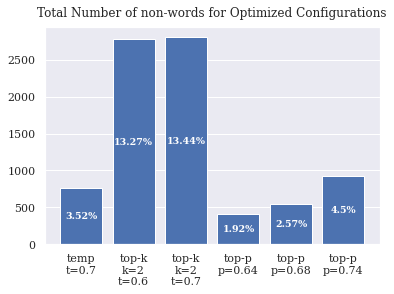
\includegraphics[scale=0.5, keepaspectratio=true]{figures/non-words.png}
    \caption{Number of Non-words for Different Configurations}
    \label{fig:non-words}
\end{figure}

Looking at \cref{fig:non-words}, it is very evident that the vast majority both of our top-k configurations are very lackluster when it comes to producing legible text. Not only are they significantly worse than our other configurations, but the sheer percentage of their generated text that consists of words, $13,65\%$ and $13.92\%$ for $k=2, t=0.6$ and $k=2, t=0.7$ respectively, is way beyond what might be deemed acceptable. This means that, for our \textit{top-k} configuration to be considered viable, it would require either the RL model itself to be more sophisticated, either through training or other measures, or the generated output would require large amounts of filtering, to ensure only verses without non-words are considered.

The figure also shows us yet another example of the trade-off that is being made to obtain higher novelty and/or rhyme density, as the lower the number of non-words a configuration produces, the lower its rhyme density consequently is. If one were to apply a filtering approach to achieve a higher quality output, it would require not only filtering out verses with low rhyme densities, but also ones that were deemed to be too incoherent, by merit of their number of non-words or other such metrics.\footnote{It should be noted that this metric is not perfect, some examples of which being that it does not account for slang words not in the vocabulary ("pimpy", "donger"), nor \textit{plausible} words ("brainin", "pussin") or many non-English words/proper nouns ("calibato"). Some of these errors might be at least partially rectified by employing a larger vocabulary to draw from, including more slang words and foreign words, but is seems unlikely to reduce the number of non-words much, and so the current version is judged sufficient}

\subsubsection{General-purpose Language Model}
\label{sec:general-purpose-lm-results}

As with the lyrics-model, the general-purpose (GP) model was parameter tuned to achieve the best possible output, which in this context meant non-repeating, coherent English text. As mentioned previously, the main objective in creating this model was to include a similarly trained baseline, on which to test the main model's proficiency on rap-specific metrics. This meant that schemes such as \textit{greedy search} and \textit{beam search} would not be explored, as the results from the initial tests, as well as previous studies \cite{HoltzmanAri2019TCCo}, has shown that they are highly unlikely to nearly be as effective as either \textit{top-k} or \textit{top-p} sampling at modelling regular language.

As an initial gauge of our GP model's proficiency at generating text, let us briefly examine some of the metrics used previously. As fewer decoding schemes have this time been included, I have chosen to increase the number of parameter configurations, including 2 of the more promising setups that we did not proceed with, after the initial parameter tuning of the RL model in \cref{chap:tuning-params}. These configurations in question are top-p, $p=0.78$ and top-k, $k=2, t=1.0$.

\begin{figure*}[ht!]
    \centering
    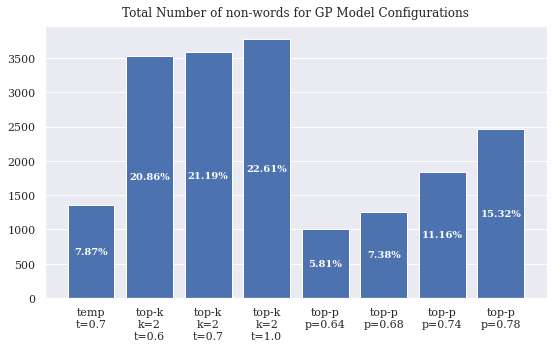
\includegraphics[scale=0.68, keepaspectratio=true]{figures/gp_non-words.png}
    \caption{Non-words for GP Model Configurations}
    \label{fig:gp_non-words}
\end{figure*}

Looking at the performance of the different configurations in \cref{fig:gp_non-words}, it is clear that all the configurations are significantly worse than their RL counterparts. The best performing configuration for the GP model is top-p $p=0.64$, which manages to "only" produce non-words 5.81\% of the time, which is still approximately 3 times higher than the 1.92\% achieved by our RL model, also with the top-p, $p=0.64$ configuration. At the other end of the spectrum, we have our top-k configurations, which still really seem to struggle to produce legible texts, though similarly significantly worse for in the case of our GP model, averaging one non-word in 1 of every 5 generated words.

\begin{table*}[ht!]
    \begin{center}
    \caption{LM Comparison - Rhyme Densities}
    \vspace{6pt}
    \label{tab:lm-comparison-rd}
    \bgroup
    \def\arraystretch{1.6}
    \resizebox{8cm}{!}{
    \begin{tabular}{|c|c|c|c|}
        \hline
        \textbf{Rank*} & \textbf{LM**} & \multicolumn{1}{c|}{\textbf{Configuration}} & \textbf{Rhyme Density} \\[0.1cm]\hline\hline
        1. (23.) & RL & Top-k, $k=2, t=0.6$ & 1.055 \\
        2. (28.) & RL & Top-k, $k=2, t=0.7$ & 1.047 \\
        3. (33.) & RL & Temp Sampling, $t=0.7$ & 1.006 \\
        4. (36.) & RL & Greedy Search & 0.994 \\
        5. (36.) & RL & Beam Search, $\beta=2$ & 0.964 \\
        6. (36.) & RL & Top-p, $p=0.64$ & 0.951 \\
        7. (36.) & RL & Top-p, $p=0.68$ & 0.947 \\
        8. (36.) & RL & Top-p, $p=0.74$ & 0.935 \\\hdashline
        9. (T36.) & GP & Top-p, $p=0.78$ & 0.924 \\
        10. (37.) & N/A & GP Dataset Baseline & 0.909 \\
        11. (37.) & GP & Top-p, $p=0.74$ & 0.885 \\
        12. (38.) & GP & Top-p, $p=0.68$ & 0.866 \\
        13. (38.) & GP & Top-p, $p=0.64$ & 0.853 \\
        14. (38.) & GP & Temp Sampling, $t=7$ & 0.826 \\
        15. (38.) & GP & Top-k, $k=2,t=0.7$ & 0.722 \\
        16. (38.) & GP & Top-k, $k=2,t=0.6$ & 0.715 \\
        17. (38.) & GP & Top-k, $k=2,t=1.0$ & 0.713 \\\hline\hline
        \multicolumn{3}{|c|}{Mean RD Difference ($L > GP$):} & \multicolumn{1}{c|}{\makecell[c]{\textbf{0.174} \\ \textbf{($\sim$21.4\%)}}} \\\hline
        \multicolumn{4}{l}{\makecell[l]{\\ * Parenthesized rank denotes the rank at which the \\ decoding configuration would have slotted in, amongst \\ all rappers}} \\
        \multicolumn{4}{l}{\makecell[l]{ ** LM = Language Model, RL = Rap Lyrics, GP = Generl-purpose.}}
    \end{tabular}
    }
    \egroup
    \end{center}
\end{table*}

To further contextualize the performance of our RL model, I have also included another parameter in \cref{tab:lm-comparison-rd}, namely the rhyme density of the GP dataset itself, providing a baseline fully comprised of real, actual English. Examining the results, we can see that every single one of our RL configurations proved to better than their GP counterparts in terms of average rhyme density, being on average $\sim$21.4\% higher. If we look at just the models that were decently successful at producing legible English text, here the three top-p configurations: $p=0.64, p=0.68$ and $p=0.74$, it is a similar story, albeit less impressive. These configurations had an average rhyme density of 0.944 for our RL model, while our GP configurations had an average rhyme density of 0.868, meaning the RL model won was 8,76\% better. Furthermore, our RL configurations also managed to perform noticeable better than the GP dataset baseline, suggesting that their attempt at mimicking rap lyrics, at least with respect to rhymes, was a success.
